\documentclass{article}
\usepackage{pgfplots}
\usepackage[most]{tcolorbox}
\usepackage{pgfplotstable}


\title{\bf{Chapter 13}\\ Principal Component Analysis}
\date{}

\begin{document}
\maketitle
\section{Problem}
Consider this plot\\

\pgfplotstableread{
  X Y
  30 6
  50 9
  60 8
  70 10
  80 12
  90 18
  100 17
  110 20
  120 22
  130 21
  140 23
  150 22
  160 24
  170 26
  180 25
  190 26
}\datatable

\begin{tabular}{|c|c|}
  \hline
  X   & Y  \\
  \hline

  30  & 6  \\
  50  & 9  \\
  60  & 8  \\
  70  & 10 \\
  80  & 12 \\
  90  & 18 \\
  100 & 17 \\
  110 & 20 \\
  120 & 22 \\
  130 & 21 \\
  140 & 23 \\
  150 & 22 \\
  160 & 24 \\
  170 & 26 \\
  180 & 25 \\
  190 & 26 \\
  \hline
\end{tabular}
$\mathbf{\Longrightarrow}$
\begin{tikzpicture}[baseline=(current bounding box.center)]
  \begin{axis}[
      xlabel={$x$},
      ylabel={$y$},
      xmin=0, xmax=200,
      ymin=0, ymax=50,
      width=8cm,
      height=6cm,
      grid=major,
      mark size = 1pt,
      legend pos=north west,
      scatter/classes={
          a={mark=o,draw=black}
        }
    ]
    \addplot [only marks, mark = *, fill=red] table {\datatable};
  \end{axis}
\end{tikzpicture}
\\\\
This data uses two dimensions to represent the information about something.\\
But do we really need 2 dimensions...?\\
and are these 2 axis(basis) the most informative..?\\
\begin{tcolorbox}[colback=blue!5!white,colframe=blue!75!black,title=Ideal Basis Properties]
  \begin{itemize}
    \item High Variance along individual basis or axis
    \item Low Covariance between basis (This means they are linearly independent)
    \item Non redundant Basis(Less Correlation between basis)
  \end{itemize}
\end{tcolorbox}
Also we are interested in represting the data using fewer dimensions such that the data has high variance along these dimensions.\\
One example would be, if the above plot was for classfication.\\
\begin{tikzpicture}[baseline=(current bounding box.center)]
  \begin{axis}[
      xlabel={$x$},
      ylabel={$y$},
      xmin=0, xmax=200,
      ymin=0, ymax=50,
      width=8cm,
      height=6cm,
      grid=major,
      mark size = 1pt,
      legend pos=north west,
      scatter/classes={
          a={mark=o,draw=black}
        }
    ]
    \addplot [only marks, mark = *, fill=red] table[x expr=(\coordindex < 6) ? \thisrow{X} : NaN, y=Y] {\datatable};
    \addplot [only marks, mark = *, fill=green] table[x expr=(\coordindex > 6) ? \thisrow{X} : NaN, y=Y] {\datatable};

  \end{axis}
\end{tikzpicture}
\\

Green points represent class A\\
Red points represent class B\\\\
Now, what if we chose some other axis instead of these x and y.\\\\
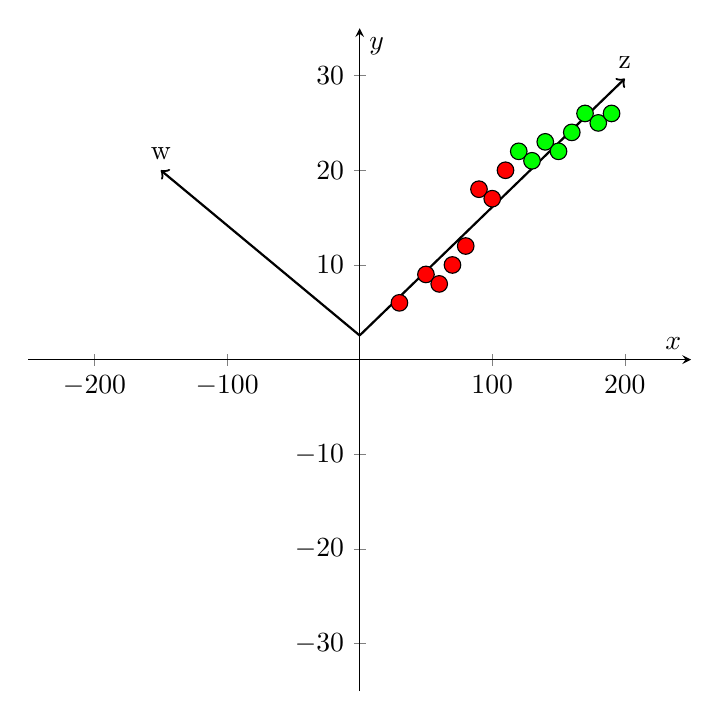
\begin{tikzpicture}
  \begin{axis}[
      width=10cm,
      height=10cm,
      xmin=-250, xmax=250,
      ymin=-35,ymax=35,
      axis lines=middle,
      xlabel=$x$,
      ylabel=$y$,
      scatter/classes={%
          a={mark=o,draw=black}}
    ]

    \addplot[scatter,only marks,
      mark size = 3pt,
      fill = red,
      scatter src=explicit symbolic] table{
        30  6
        50  9
        60  8
        70  10
        80  12
        90  18
        100 17
        110 20
      };
    \addplot[scatter,only marks,
      mark size = 3pt,
      fill = green,
      scatter src=explicit symbolic] table{
        120 22
        130 21
        140 23
        150 22
        160 24
        170 26
        180 25
        190 26
      };
    \draw[->,thick] (axis cs:0, 2.556) -- (axis cs:200,29.676) node[pos=1,above]{z};
    \draw[->,thick] (axis cs:0, 2.556) -- (axis cs:-150,20) node[pos=1,above]{w};
  \end{axis}
\end{tikzpicture}
\\
On this new z axis, all points seem to lie pretty close to it, with negligible variance along the w axis\\
and since this data was for classification, we can actually represent this 2D data in just 1 Dimension on Z axis\\

\section{Setup}
Let $p_1,p_2,p_3,\dots,p_n$ be a set of linearly independent orthonormal vectors.\\
These are going to be our new ideal basis vectors.\\
Let P be n x n matrix such that $p_1,p_2,p_3,\dots,p_n$ are the columns of P.
$$
  P=\begin{bmatrix}
    \uparrow   & \uparrow   & \dots & \uparrow   \\
    p_1        & p_2        & \dots & p_n        \\
    \downarrow & \downarrow & \dots & \downarrow \\
  \end{bmatrix}
$$
Let $x_1,x_2,\dots,x_m\in R^n$ be the sample vectors of size (n x 1) from the database of m data points.\\
X is the matrix such that $x_1,x_2,\dots,x_m$ are the columns of it.\\
$$
  X=\begin{bmatrix}
    \uparrow   & \uparrow   & \dots & \uparrow   \\
    x_1        & x_2        & \dots & x_m        \\
    \downarrow & \downarrow & \dots & \downarrow \\
  \end{bmatrix}
$$
Further let us assume that the data is 0-mean and unit-variance.\\
\section{Finding the ideal basis}

Let us assume currently the basis of $x_{ij}$ is $\hat{b_{j}}$\\
Hence,\\
$$
  x_i=x_{i1}\hat{b_1}+x_{i2}\hat{b_2}+\dots+x_{in}\hat{b_n}
$$
Since P is the matrix of new basis.\\
This means each vector of X can be written as a linear combination of these new basis vectors\\
$$
  x_i=\alpha_{i1}.p_1+\alpha_{i2}.p_2+\dots+\alpha_{in}.p_n
$$
$$
  x_i=\begin{bmatrix}
    \alpha_{i1} \\
    \alpha_{i2} \\
    \vdots      \\
    \alpha_{in} \\
  \end{bmatrix}
$$
and for orthonormal basis we know that we can find $\alpha_i$'s using\\
$$
  \alpha_{ij}=x_i^T \cdot p_j
$$
$$
  \alpha_{ij}=\begin{bmatrix}
    x_{i1} &
    x_{i2} &
    \dots  &
    x_{in}\\
  \end{bmatrix} \cdot \begin{bmatrix}
    p_{j1} \\
    p_{j2} \\
    \vdots \\
    p_{jn} \\
  \end{bmatrix}
$$

Hence,\\
$$
  \hat{x_i}=\begin{bmatrix}
    x_i^T \cdot p_1 \\
    x_i^T \cdot p_2 \\
    \vdots          \\
    x_i^T \cdot p_n \\
  \end{bmatrix}=\begin{bmatrix}
    \mathbf{\longleftarrow } & x_i & \mathbf{\longrightarrow} \\
  \end{bmatrix} \cdot \begin{bmatrix}
    p_1    \\
    p_2    \\
    \vdots \\
    p_n    \\
  \end{bmatrix}=\begin{bmatrix}
    \mathbf{\longleftarrow } & x_i & \mathbf{\longrightarrow} \\
  \end{bmatrix} \cdot \begin{bmatrix}
    \uparrow   & \uparrow   & \dots & \uparrow   \\
    p_1        & p_2        & \dots & p_n        \\
    \downarrow & \downarrow & \dots & \downarrow \\
  \end{bmatrix}
$$
So, any vector new basis would look like\\
$$
  \hat{x_i}=x_i^T \cdot P
$$

All the vectors would look like\\
$$
  \hat{X}=\begin{bmatrix}
    \uparrow   & \uparrow   & \dots & \uparrow   \\
    \hat{x_1}  & \hat{x_2}  & \dots & \hat{x_m}  \\
    \downarrow & \downarrow & \dots & \downarrow \\
  \end{bmatrix}=\begin{bmatrix}
    \uparrow   & \uparrow   & \dots & \uparrow   \\
    x_1^T.P    & x_2^T.P    & \dots & x_m^T.P    \\
    \downarrow & \downarrow & \dots & \downarrow \\
  \end{bmatrix}=\begin{bmatrix}
    \uparrow   & \uparrow   & \dots & \uparrow   \\
    x_1^T      & x_2^T      & \dots & x_m^T      \\
    \downarrow & \downarrow & \dots & \downarrow \\
  \end{bmatrix}.\begin{bmatrix}
    \uparrow   & \uparrow   & \dots & \uparrow   \\
    p_1        & p_2        & \dots & p_m        \\
    \downarrow & \downarrow & \dots & \downarrow \\
  \end{bmatrix}
$$
$$
  \hat{X}=X \cdot P
$$
\textbf{Theorem:}\\
If X is a matrix such that its column has zero mean and if $\hat{X}=XP$ then columns of $\hat{X}$ would also have zero mean.\\

\textbf{Theorem:}\\
If X is a matrix whose columns have zero mean then $\Sigma=\frac{X^TX}{m}$ is the Covariance matrix.\\
$\Sigma_{i,j}$ stores the covariance between $x_i$ and $x_j$
$$
  \Sigma=\frac{\begin{bmatrix}
      \mathbf{\longleftarrow} & x_1 & \mathbf{\longrightarrow} \\
      \mathbf{\longleftarrow} & x_2 & \mathbf{\longrightarrow} \\
      \vdots\\
      \mathbf{\longleftarrow} & x_m & \mathbf{\longrightarrow} \\
    \end{bmatrix}.\begin{bmatrix}
      \uparrow   & \uparrow   & \dots & \uparrow   \\
      x_1        & x_2        & \dots & x_m        \\
      \downarrow & \downarrow & \dots & \downarrow \\
    \end{bmatrix}}{m}=\frac{\begin{bmatrix}
      \mathbf{\longleftarrow}x_1.x_1\mathbf{\longrightarrow} & \mathbf{\longleftarrow}x_1.x_2\mathbf{\longrightarrow} & \dots  & \mathbf{\longleftarrow}x_1.x_m\mathbf{\longrightarrow} \\
      \mathbf{\longleftarrow}x_2.x_1\mathbf{\longrightarrow} & \mathbf{\longleftarrow}x_2.x_2\mathbf{\longrightarrow} & \dots  & \mathbf{\longleftarrow}x_2.x_m\mathbf{\longrightarrow} \\
      \vdots                                                 & \vdots                                                 & \ddots & \vdots                                                 \\
      \mathbf{\longleftarrow}x_m.x_1\mathbf{\longrightarrow} & \mathbf{\longleftarrow}x_m.x_2\mathbf{\longrightarrow} & \dots  & \mathbf{\longleftarrow}x_m.x_m\mathbf{\longrightarrow} \\
    \end{bmatrix}}{m}
$$
$$
  \Sigma=\begin{bmatrix}
    Cov(x_1,x_1) & Cov(x_1,x_2) & \dots  & Cov(x_1,x_m) \\
    Cov(x_2,x_1) & Cov(x_2,x_2) & \dots  & Cov(x_2,x_m) \\
    \vdots       & \vdots       & \ddots & \vdots       \\
    Cov(x_m,x_1) & Cov(x_m,x_2) & \dots  & Cov(x_m,x_m) \\
  \end{bmatrix}
$$
\pagebreak

Since $\hat{X}$ is the data with new basis\\\\
Covariance matrix of $\hat{X}=\frac{\hat{X}^T.\hat{X}}{m}$\\
$$
  \frac{\hat{X}^T.\hat{X}}{m}=\frac{(X.P)^T.(X.P)}{m}=P^T.\frac{(X^T.X)}{m}.P=P^T\Sigma P
$$
Ok, we want basis vectors to be linearly independent, this means all basis vectors should have 0 covariance and we also want vectors to have non-zero variance with itself.\\
\begin{tcolorbox}[colback=blue!5!white,colframe=blue!75!black,title=Ideal Basis Properties]
  \begin{itemize}
    \item $\left(\frac{\hat{X}^T.\hat{X}}{m}\right)_{(i,j)}$=0 if i$\neq$ j, meaning low covariance
    \item $\left(\frac{\hat{X}^T.\hat{X}}{m}\right)_{(i,j)}\neq$0 if i=j, meaning non-zero variance
  \end{itemize}
\end{tcolorbox}
Hence,\\
$$
  \frac{\hat{X}^T.\hat{X}}{m}=\begin{bmatrix}
    Cov(\hat{x_1},\hat{x_1}) & Cov(\hat{x_1},\hat{x_2}) & \dots  & Cov(\hat{x_1},\hat{x_m}) \\
    Cov(\hat{x_2},\hat{x_1}) & Cov(\hat{x_2},\hat{x_2}) & \dots  & Cov(\hat{x_2},\hat{x_m}) \\
    \vdots                   & \vdots                   & \ddots & \vdots                   \\
    Cov(\hat{x_m},\hat{x_1}) & Cov(\hat{x_m},\hat{x_2}) & \dots  & Cov(\hat{x_m},\hat{x_m}) \\
  \end{bmatrix}
$$
will become\\
$$
  \frac{\hat{X}^T.\hat{X}}{m}=\begin{bmatrix}
    Cov(x_1,x_1) & 0            & \dots  & 0            \\
    0            & Cov(x_2,x_2) & \dots  & 0            \\
    \vdots       & \vdots       & \ddots & \vdots       \\
    0            & 0            & \dots  & Cov(x_m,x_m) \\
  \end{bmatrix}
$$

This means\\\\
\pagebreak

$\frac{\hat{X}^T.\hat{X}}{m}=P^T\Sigma P$ is a Diagonal matrix.\\\\
And we know,\\
$\Sigma$ is a Square matrix\\
$P$ is an orthogonal matrix\\\\
The questions is, Which orthogonal matrix can diagonalise $\Sigma$?\\
Answer is, a matrix whose columns are eigenvectors of $\Sigma$.\\\\
Also,\\
$$
  P^T\Sigma P=\Lambda
$$
Here $\Lambda$ is a diagonal matrix containing Eigen-values of $\Sigma$ matrix.\\
$$
  P=\begin{bmatrix}
    \uparrow   & \uparrow   & \dots & \uparrow   \\
    \vec{v_1}  & \vec{v_2}  & \dots & \vec{v_n}  \\
    \downarrow & \downarrow & \dots & \downarrow \\
  \end{bmatrix}
$$
Here, $\vec{v_1}, \vec{v_2}, \dots , \vec{v_n}$ are the eigenvectors of $\Sigma$.\\\\
Hence, we found the ideal basis vector values with these properties.
\begin{tcolorbox}[colback=blue!5!white,colframe=blue!75!black,title=Ideal Basis Properties]
  \begin{itemize}
    \item High Variance along individual basis or axis
    \item Low Covariance between basis (This means they are linearly independent)
    \item Non redundant Basis(Less Correlation between basis)
  \end{itemize}
\end{tcolorbox}
That is, the new basis P used to transform X is the basis consisting of Eigenvectors of $X^TX$\\

This method is called Principal Component Analysis for transforming the data to a new basis where the dimensions are non-redundant(low-covariance) \& not noisy(high variance).

\end{document}
